\documentclass[11pt,a4paper]{article}
\pdfoutput=1
\usepackage{jheppub}
\usepackage{bbm}
\usepackage{youngtab}
\usepackage{graphicx, wrapfig}
\usepackage{rotfloat}
\usepackage{stmaryrd}
\usepackage{amsfonts,amssymb,amsmath,mathtools}
\usepackage{mathrsfs}
\usepackage{tikz}
\usepackage{shadow}
\usepackage{fancybox}
\usepackage{xcolor}
\usepackage{float}
\usepackage[all,cmtip]{xy}
\usepackage{slashed}


%%%%%%%%%%%% MACROS  MACROS   MACROS %%%%%%%%%


 \usetikzlibrary{decorations.markings}
\newcommand{\maplr}[2]{\begin{picture}(40,20)(0,20)
    \put(18,32){{\small $#1$}}
    \put(3,25){\vector(1,0){34}}
    \put(37,20){\vector(-1,0){34}}
     \put(18,10){{\small $#2$}}
  \end{picture}
}

%%%%%%%%%%%% Maths theorem environments  %%%%%%%%%


\newenvironment{theorem}{\begin{quote} \footnotesize }{ \normalsize \end{quote}}

\newtheorem{thm}{Theorem}[section]
\newtheorem{corollary}{Corollary}[section]
\newtheorem{lemma}[section]{Lemma}
\newtheorem{proposition}{Proposition}[section]
\newtheorem{example}{Example}



%%%%%%%  Better lists %%%%%%%%%%%%%%%%%%
\newenvironment{myenumerate}{
\begin{enumerate}
   \setlength{\itemsep}{1pt}
   \setlength{\parskip}{0pt}
   \setlength{\parsep}{0pt}}{\end{enumerate}}
\newenvironment{myitemize}{
\begin{description}

   \setlength{\itemsep}{1pt}
   \setlength{\parskip}{0pt}
   \setlength{\parsep}{0pt}}{\end{description}
}

\renewcommand{\labelenumii}{\arabic{enumi}-\roman{enumii}}

%%%%%%%  Greek letters %%%%%%%%%%%%%%%%%%
\def\a{\alpha}
\def\b{\beta}
\def\c{\gamma} \def\g{\gamma}
\def\d{\delta}
\def\e{\epsilon}
\def\f{\phi}
\def\vf{\varphi}  \def\tvf{\tilde{\varphi}}
\def\vp{\varphi}
\def\h{\eta}
\def\i{\iota}
\def\j{\psi}
\def\k{\kappa}
\def\m{\mu}
\def\n{\nu}
\def\o{\omega}  \def\w{\omega}
\def\q{\theta}  \def\th{\theta}
\def\r{\rho}
\def\s{\sigma}
\def\t{\tau}
\def\u{\upsilon}
\def\x{\xi}
\def\z{\zeta}

\def\A{\Alpha}
\def\B{\Beta}
\def\G{\Gamma}
\def\D{\Delta}
\def\E{\Epsilon}
\def\F{Phi}
\def\h{\eta}
\def\I{\Iota}
\def\J{Psi}
\def\K{\Kappa}
\def\L{\Lambda}
\def\M{\Mu}
\def\N{\Nu}
\def\O{\Omega}  \def\w{\omega}
\def\Q{\Theta}  \def\Th{\Theta}
\def\R{\Rho}
\def\Si{\Sigma}
\def\T{\Tau}
\def\Up{\Upsilon}
\def\X{\Xi}
\def\Z{\Zeta}

\DeclareMathOperator{\id}{id}
\DeclareMathOperator{\Hom}{Hom}
\DeclareMathOperator{\Mat}{Mat}
\DeclareMathOperator{\rk}{rk}
%%%%%%%%%%%% math fonts %%%%%%%%%%%%%%%%%%%%%%%%%%%%%%%%%%%%%
%
%---------- mathbb font --------------------------------
%

\newcommand{\bA}{\ensuremath{\mathbb{A}}}
\newcommand{\bB}{\ensuremath{\mathbb{B}}}
\newcommand{\bC}{\ensuremath{\mathbb{C}}}
\newcommand{\bD}{\ensuremath{\mathbb{D}}}
\newcommand{\bE}{\ensuremath{\mathbb{E}}}
\newcommand{\bF}{\ensuremath{\mathbb{F}}}
\newcommand{\bG}{\ensuremath{\mathbb{G}}}
\newcommand{\bH}{\ensuremath{\mathbb{H}}}
\newcommand{\bI}{\ensuremath{\mathbb{I}}}
\newcommand{\bJ}{\ensuremath{\mathbb{J}}}
\newcommand{\bK}{\ensuremath{\mathbb{K}}}
\newcommand{\bL}{\ensuremath{\mathbb{L}}}
\newcommand{\bM}{\ensuremath{\mathbb{M}}}
\newcommand{\bN}{\ensuremath{\mathbb{N}}}
\newcommand{\bO}{\ensuremath{\mathbb{O}}}
\newcommand{\bP}{\ensuremath{\mathbb{P}}}
\newcommand{\bQ}{\ensuremath{\mathbb{Q}}}
\newcommand{\bR}{\ensuremath{\mathbb{R}}}
\newcommand{\bS}{\ensuremath{\mathbb{S}}}
\newcommand{\bT}{\ensuremath{\mathbb{T}}}
\newcommand{\bU}{\ensuremath{\mathbb{U}}}
\newcommand{\bV}{\ensuremath{\mathbb{V}}}
\newcommand{\bW}{\ensuremath{\mathbb{W}}}
\newcommand{\bX}{\ensuremath{\mathbb{X}}}
\newcommand{\bY}{\ensuremath{\mathbb{Y}}}
\newcommand{\bZ}{\ensuremath{\mathbb{Z}}}


%
%---------- mathscript font -----------------------------
%

\newcommand{\scA}{\ensuremath{\mathscr{A}}}
\newcommand{\scB}{\ensuremath{\mathscr{B}}}
\newcommand{\scC}{\ensuremath{\mathscr{C}}}
\newcommand{\scD}{\ensuremath{\mathscr{D}}}
\newcommand{\scE}{\ensuremath{\mathscr{E}}}
\newcommand{\scF}{\ensuremath{\mathscr{F}}}
\newcommand{\scG}{\ensuremath{\mathscr{G}}}
\newcommand{\scH}{\ensuremath{\mathscr{H}}}
\newcommand{\scI}{\ensuremath{\mathscr{I}}}
\newcommand{\scJ}{\ensuremath{\mathscr{J}}}
\newcommand{\scK}{\ensuremath{\mathscr{K}}}
\newcommand{\scL}{\ensuremath{\mathscr{L}}}
\newcommand{\scM}{\ensuremath{\mathscr{M}}}
\newcommand{\scN}{\ensuremath{\mathscr{N}}}
\newcommand{\scO}{\ensuremath{\mathscr{O}}}
\newcommand{\scP}{\ensuremath{\mathscr{P}}}
\newcommand{\scQ}{\ensuremath{\mathscr{Q}}}
\newcommand{\scR}{\ensuremath{\mathscr{R}}}
\newcommand{\scS}{\ensuremath{\mathscr{S}}}
\newcommand{\scT}{\ensuremath{\mathscr{T}}}
\newcommand{\scU}{\ensuremath{\mathscr{U}}}
\newcommand{\scV}{\ensuremath{\mathscr{V}}}
\newcommand{\scW}{\ensuremath{\mathscr{W}}}
\newcommand{\scX}{\ensuremath{\mathscr{X}}}
\newcommand{\scY}{\ensuremath{\mathscr{Y}}}
\newcommand{\scZ}{\ensuremath{\mathscr{Z}}}
\newcommand{\scAH}{\ensuremath{\mathscr{A}\!\!\scH}}

%
%---------- mathfrak font -----------------------------
%

\newcommand{\frakA}{\ensuremath{\mathfrak{A}}}
\newcommand{\frakB}{\ensuremath{\mathfrak{B}}}
\newcommand{\frakC}{\ensuremath{\mathfrak{C}}}
\newcommand{\frakD}{\ensuremath{\mathfrak{D}}}
\newcommand{\frakE}{\ensuremath{\mathfrak{E}}}
\newcommand{\frakF}{\ensuremath{\mathfrak{F}}}
\newcommand{\frakG}{\ensuremath{\mathfrak{G}}}
\newcommand{\frakH}{\ensuremath{\mathfrak{H}}}
\newcommand{\frakI}{\ensuremath{\mathfrak{I}}}
\newcommand{\frakJ}{\ensuremath{\mathfrak{J}}}
\newcommand{\frakK}{\ensuremath{\mathfrak{K}}}
\newcommand{\frakL}{\ensuremath{\mathfrak{L}}}
\newcommand{\frakM}{\ensuremath{\mathfrak{M}}}
\newcommand{\frakN}{\ensuremath{\mathfrak{N}}}
\newcommand{\frakO}{\ensuremath{\mathfrak{O}}}
\newcommand{\frakP}{\ensuremath{\mathfrak{P}}}
\newcommand{\frakQ}{\ensuremath{\mathfrak{Q}}}
\newcommand{\frakR}{\ensuremath{\mathfrak{R}}}
\newcommand{\frakS}{\ensuremath{\mathfrak{S}}}
\newcommand{\frakT}{\ensuremath{\mathfrak{T}}}
\newcommand{\frakU}{\ensuremath{\mathfrak{U}}}
\newcommand{\frakV}{\ensuremath{\mathfrak{V}}}
\newcommand{\frakW}{\ensuremath{\mathfrak{W}}}
\newcommand{\frakX}{\ensuremath{\mathfrak{X}}}
\newcommand{\frakY}{\ensuremath{\mathfrak{Y}}}
\newcommand{\frakZ}{\ensuremath{\mathfrak{Z}}}
\newcommand{\fraka}{\ensuremath{\mathfrak{a}}}
\newcommand{\frakb}{\ensuremath{\mathfrak{b}}}
\newcommand{\frakc}{\ensuremath{\mathfrak{c}}}
\newcommand{\frakd}{\ensuremath{\mathfrak{d}}}
\newcommand{\frake}{\ensuremath{\mathfrak{e}}}
\newcommand{\frakf}{\ensuremath{\mathfrak{f}}}
\newcommand{\frakg}{\ensuremath{\mathfrak{g}}}
\newcommand{\frakh}{\ensuremath{\mathfrak{h}}}
\newcommand{\fraki}{\ensuremath{\mathfrak{i}}}
\newcommand{\frakj}{\ensuremath{\mathfrak{j}}}
\newcommand{\frakk}{\ensuremath{\mathfrak{k}}}
\newcommand{\frakl}{\ensuremath{\mathfrak{l}}}
\newcommand{\frakm}{\ensuremath{\mathfrak{m}}}
\newcommand{\frakn}{\ensuremath{\mathfrak{n}}}
\newcommand{\frako}{\ensuremath{\mathfrak{o}}}
\newcommand{\frakp}{\ensuremath{\mathfrak{p}}}
\newcommand{\frakq}{\ensuremath{\mathfrak{q}}}
\newcommand{\frakr}{\ensuremath{\mathfrak{r}}}
\newcommand{\fraks}{\ensuremath{\mathfrak{s}}}
\newcommand{\frakt}{\ensuremath{\mathfrak{t}}}
\newcommand{\fraku}{\ensuremath{\mathfrak{u}}}
\newcommand{\frakv}{\ensuremath{\mathfrak{v}}}
\newcommand{\frakw}{\ensuremath{\mathfrak{w}}}
\newcommand{\frakx}{\ensuremath{\mathfrak{x}}}
\newcommand{\fraky}{\ensuremath{\mathfrak{y}}}
\newcommand{\frakz}{\ensuremath{\mathfrak{z}}}
\newcommand{\fraksl}{\ensuremath{\mathfrak{sl}}}
\newcommand{\frakso}{\ensuremath{\mathfrak{so}}}
\newcommand{\fraksp}{\ensuremath{\mathfrak{sp}}}

%%%%%%%%%%%%  Calligraphic, Roman and Maths integers %%%%%%%%%%%%%%%%%%

\newcommand{\cA}{\mathcal{A}}
\newcommand{\cB}{\mathcal{B}}
\newcommand{\cC}{\mathcal{C}}
\newcommand{\cD}{\mathcal{D}}
\newcommand{\cE}{\mathcal{E}}
\newcommand{\cF}{\mathcal{F}}
\newcommand{\cG}{\mathcal{G}}
\newcommand{\cH}{\mathcal{H}}
\newcommand{\cI}{\mathcal{I}}
\newcommand{\cJ}{\mathcal{J}}
\newcommand{\cK}{\mathcal{K}}
\newcommand{\cL}{\mathcal{L}}
\newcommand{\cM}{\mathcal{M}}
\newcommand{\cN}{\mathcal{N}}
\newcommand{\cO}{\mathcal{O}}
\newcommand{\cQ}{\mathcal{Q}}
\newcommand{\cS}{\mathcal{S}}
\newcommand{\cX}{\mathcal{X}}
\newcommand{\cY}{\mathcal{Y}}
\newcommand{\cW}{\mathcal{W}}
\newcommand{\cR}{\mathcal{R}}
\newcommand{\cT}{\mathcal{T}}
\newcommand{\cZ}{\mathcal{Z}}

%%%%%%%%%%%%%%%%%%%%%%%%%%%%%%%%%%%%%%%%%%%%%%%%%%%%%%%%%%%%%%%%
\newcommand{\SU}{\mathrm{SU}}
\newcommand{\SO}{\mathrm{SO}}
\newcommand{\SL}{\mathrm{SL}}
\newcommand{\Sp}{\mathrm{Sp}}
\newcommand{\su}{\mathrm{su}}
\newcommand{\so}{\mathrm{so}}
\newcommand{\spl}{\mathrm{sp}}
\newcommand{\gl}{\mathrm{gl}}
\newcommand{\sll}{\mathrm{sl}}
\newcommand{\U}{\mathrm{U}}
\newcommand{\ul}{\mathrm{u}}
\newcommand{\Spin}{\mathrm{Spin}}
\newcommand{\Pin}{\mathrm{Pin}}
%%%%%%%%%%%%%%%%%%%%%%%%%%%%%%%%%%%%%%%%%%%%%%%%%%%%%%%%%%%%%%%%
\renewcommand{\Im}{{\rm Im}}
\renewcommand{\Re}{{\rm Re}}
\newcommand{\Tr}{\mbox{Tr}}
\newcommand{\Pf}{\mbox{Pf}}
\newcommand{\sgn}{\mbox{sgn}}
\newcommand{\Vir}{{\rm Vir}}
\newcommand{\Li}{{\rm Li}}


\def\CP{\mathbb{CP}}
%\def\cD{{\cal D}}
%\def\cA{{\cal A}}
%\def\cN{{\cal N}}
%\def\cS{{\cal S}}
%\def\cD{{\cal D}}
%\def\cA{{\cal A}}
%%%%%%%%%%%%%%%%%%%%%%%%%%%%%%%%%%%%%%%%%%%%%%%%%%%%%%%%%%%%%%%%


\newcommand{\valp}{{\vec\alpha}}
\newcommand{\vbet}{{\vec\beta}}
\newcommand{\vgam}{{\vec\gamma}}
\newcommand{\vrho}{{\vec\rho}}
\newcommand{\vome}{{\vec\omega}}
\newcommand{\vlam}{{\vec\lambda}}
\newcommand{\vphi}{{\vec\varphi}}
\newcommand{\va}{{\vec a}}
\newcommand{\vb}{{\vec b}}
\newcommand{\ve}{{\vec e}}
\newcommand{\vx}{{\vec x}}
\newcommand{\vW}{{\vec W}}
\newcommand{\vY}{{\vec Y}}
\newcommand{\vha}{{\vec{\hat a}}}
\newcommand{\vhb}{{\vec{\hat b}}}
\newcommand{\vhc}{{\vec{\hat c}}}

%%%%%%%%%%%%%%%%%%%%%%%%%%%%%%%%%%%%%%%%%%%%%%%%%%%%%%%%%%%%%%%%



\newcommand{\dalpha}{{\dot \alpha}}
\newcommand{\dbeta}{{\dot \beta}}
\newcommand{\dgamma}{{\dot \gamma}}
\newcommand{\dmu}{{\dot \mu}}
\newcommand{\dnu}{{\dot \nu}}
\newcommand{\drho}{{\dot \rho}}
\newcommand{\dsigma}{{\dot \sigma}}
\newcommand{\dlambda}{{\dot \lambda}}
\newcommand{\dtau}{{\dot \tau}}
\newcommand{\ha}{{\hat a}}
\newcommand{\hb}{{\hat b}}
\newcommand{\hc}{{\hat c}}
\newcommand{\hj}{j^\circ}
\newcommand{\vh}{{\vec h}}
\newcommand{\vm}{{\vec m}}
\newcommand{\vn}{{\vec n}}
\newcommand{\vl}{{\vec l}}





%%%%%%%  Mathmode commands %%%%%%%%%%%%%%%%%%
\newcommand{\HFK}{\widehat{\mathit{HFK}}}
\newcommand{\hfhat}{\widehat{\mathit{HF}}}
\newcommand{\hfk}{\mathit{HFK}}
\newcommand{\WL}{{\rm  \textbf{WL}}}
\newcommand{\BR}{{\rm  \textbf{BR}}}
\newcommand{\fin}{{\:\rm  fin}}
\newcommand{\vslash}{\ensuremath \raisebox{0.025cm}{\slash}\hspace{-0.21cm} v}
\newcommand{\nslash}{\ensuremath \raisebox{0.025cm}{\slash}\hspace{-0.25cm} \nabla}
\newcommand{\Dslash}{\; \ensuremath \raisebox{0.03cm}{\slash}\hspace{-0.28cm} D}
\newcommand{\Eslash}{\; \ensuremath \raisebox{0.025cm}{\slash}\hspace{-0.28cm} E}
\newcommand{\slashD}{\hat{\ensuremath \raisebox{0.025cm}{\slash}\hspace{-0.28cm} {\cal D}}}
%\DeclareMathOperator{\Mat}{Mat}

\newcommand{\half}{\frac{1}{2}}
\newcommand{\ndt}{\noindent}


\newcommand{\pa}{\partial}
\newcommand{\pab}{\bar{\partial}}
\newcommand{\nn}{\nonumber}
%
%\newcommand{\0}{{\scriptscriptstyle{(0)}}}
%\newcommand{\1}{{\scriptscriptstyle{(1)}}}
%\newcommand{\2}{{\scriptscriptstyle{(2)}}}


\newcommand{\HOMFLY}{{\rm HOMFLY}}
\newcommand{\Kauffman}{{\rm Kauff}}
\newcommand{\univ}{{\rm univ}}
\newcommand{\thin}{{\rm thin}}


\newcommand{\tia}{\tilde{a}}
\newcommand{\tI}{\tilde{I} }
\newcommand{\tell}{\tilde{\ell}}
\newcommand{\tY}{\tilde{Y}}
\newcommand{\tij}{\tilde{\jmath}}
\def\Lt{{\tilde L}}
\def\e{\epsilon}
\def\dt{\!\cdot\!}
\def\i{\mathrm{i}}

\newcommand{\brp}{{\bar p}}
\newcommand{\bmu}{{\bar\mu}}

\newcommand{\cdotsb}{\cdots{\;\!\!}}

%\def\IC{\mathbb{C}}
%\def\IP{\mathbb{P}}
%\def\IT{\mathbb{T}}

%\def\Tr{{ \rm Tr}}


\def\p{\partial}
%\def\be{\begin{equation}}
%\def\ee{\end{equation}}
%\def\bea{\begin{eqnarray}}
%\def\eea{\end{eqnarray}}



\def\bea{\begin{eqnarray}}
\def\eea{\end{eqnarray}}
\def\be{\begin{equation}}
\def\ee{\end{equation}}
\def\ba{\begin{align}}
\def\ea{\end{align}}


\newcommand{\bem}{\begin{pmatrix}}
\newcommand{\eem}{\end{pmatrix}}

\def\ib{{\bar i}}
\def\zb {\bar{z}}
\def\mb {\bar{m}}
 \def\nb {\bar{n}}
\def\wb {\bar{w}}
\def\qb {\bar{q}}



\def\={\;  = \;}
%\newcommand{\=}{\;  = \;}
\def\+{\, + \,}

\def\tl{\tilde}
\def\wt{\widetilde}
\def\wh{\widehat}
\def\bar{\overline}

\def\rt2{\sqrt{2}}

%\newcommand{\e}{\mathrm{e}}
\def\diff{{\rm diff}}
\def\Diff{{\rm Diff}}
\def\Dt{{\rm Det}}

\newcommand{\tx}{\text}
\DeclareMathOperator*{\Res}{Res}



\newcommand{\unknot}{{\raisebox{-.11cm}{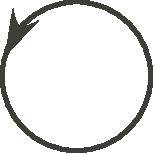
\includegraphics[width=.37cm]{unknot.pdf}}}\,}


%% These below already exist in AMS
%\def\Tr{{\rm Tr}}
%\def\lim{{\rm lim}}
%\def\mod{{\rm mod}}

\def\gpg{g^{-1} \p g}
\def\bb#1#2{\left\llbracket\begin{array}{c}{#1}\\{#2}\end{array}\right\rrbracket}


\renewcommand{\Im}{\mbox{Im}}
\renewcommand{\Re}{\mbox{Re}}

\newcommand{\BesselI}[3]{\hat I_{#1}\left( #2 \pi \sqrt{ #3 }\right)}

\newcommand{\Zar}[2]{Z\!\left[ {}^{#1}_{#2} \right]}

%\newcommand{\ar}[2]{\left[ {}^{#1}_{#2} \right]}
%\newcommand{\art}[2]{\left[ {}^{\frac{#1}{2}}_{\frac{#2}{2}}
%\right]}


\def\vt#1#2#3{ {\vartheta[{#1 \atop  #2}](#3\vert \tau)} }





%%% MY COMMENTS



\newcommand{\MyRed}{\color [rgb]{0.9,0,0}}
\newcommand{\MyGreen}{\color [rgb]{0,0.5,0}}
\newcommand{\MyBlue}{\color [rgb]{0,0,0.8}}
\newcommand{\MyBrown}{\color [rgb]{0.8,0.3,0.2}}
\newcommand{\MyPurple}{\color [rgb]{0.6,0.0,0.7}}

\def\SG#1{{\MyBlue [SG: #1]}}
\def\SN#1{{\MyBrown [SN: #1]}}
\def\MS#1{{\MyGreen [MS: #1]}}
\def\PS#1{{\MyPurple [PS: #1]}}


\begin{document}

\section{Introduction}
\subsection{Toward quantum theory of  gravity}

What is string theory and why should we study it? Current understanding of elementary constituents of matters are described by standard model (Glashow-Weingberg-Salam model). It is constructed based on QFT, which is generalization of QED. In QED, we have electron, which is described by Dirac field $\psi$, photon, which is described by gauge fields $A_\mu$ where the action is written as
$$
S=\int d^4 x \left[\bar\psi\slashed{D}\psi+\frac14F\wedge \ast F\right]~.
$$
On can generalize it to QCD by introducing lepton, non-Abelian gauge fields
$$
\textrm{quarks}: \begin{matrix} u & c  & t\\d & s & b\end{matrix}~,\quad  \textrm{leptons}: \begin{matrix} e & \mu  & \tau\\\nu_e & \nu_\mu & \nu_\tau\end{matrix}~,\qquad \textrm{gauge fields} :A_\mu~, \ G_\mu^a~, \ W_\mu^\pm,Z_\mu
$$
as well as Higgs fields $\phi$.

The problem arises when we include gravity to the Standard Model. The gravity is an important force at long (terrestrial) distances. The theory of gravity is described by General Relativity whose non-relativistic limit with weak gravitational field reduces to Newtonian gravity. Every known object gravitates so that their constituent elementary particles must also gravitate. however the interactions among elementary particles described by the Standard Model does not include gravity. 

When is the SM so successful in explaining observed experimental results? It is easy to compare gravitational and electromagnetic force between two protons
$$
\frac{G_N m_p^2/r^2}{e_p^2/r^2}=\frac{G_N m_p^2}{e_p^2}\simeq 10^{-36}~.
$$
so that the gravitational force is much weaker than electromagnetic and other forces. Nevertheless, however small it may be, gravitational interaction is certainly present in nature and must be included in a complete theory. Also, gravitational interaction does not always remain small. Let us consider two protons colliding to each other with large energy of order $E$. Effective mass of each proton is $E/c^2$ so that gravitational interaction between two protons get magnified by a factor of $(E/(m_pc^2))^2$. Although the EM interaction between two protons also grows with $E$, it grows only longitudinally $\sim\ln (E/(m_pc^2))$. If $E/(m_pc^2)\sim 10^{19}$, then the gravitational and EM interaction become comparable. Result of such an experiment cannot be predicted by the SM. Note that at present we cannot carry out this experiment due to lack of powerful enough accelerators. However a complete theory must be able to predict two results of all experiments including these which cannot be performed due to practical limitation. Conclusion is a complete theory must include the effect of gravitational interaction between elementary particles. 

What do we know about gravity? Classical gravity is described by General Relativity. In GR, dynamical variable is metric $g_{\mu\nu} (\vec x,t)$ describing geometry of space time, which satisfy 
$$
{\displaystyle R_{\mu \nu }-{\tfrac {1}{2}}R\,g_{\mu \nu }+\Lambda g_{\mu \nu }={\frac {8\pi G}{c^{4}}}T_{\mu \nu }}
$$

GR is a classical field theory with $g_{\mu\nu}(\vec x,t)$ as the classical fields. In contract, the SM is a QFT with quarks and lepton fields, gauge fields etc as dynamical fields. At present there is no direct experimental evidence that gravity satisfies the rules of QM. Could it be that the complete theory is just a combination of the SM and classical GR? This is not possible since elementary particles like electrons, which are known to obey the laws of QM, act as the source of gravity. Note that an electron produces gravitational field and if we could measure all components of the metric and their time derivatives exactly, then we could reconstruct the position and momentum of two electron to  arbitrary accuracy. This will violate the rules of quantum mechanics for the electron. Gravity must also satisfy the rules of QM, i.e. these should be an uncertainty principle involving the measurement of the metric and its time derivative. 

As an aside, the same argument may be used to show that the EM field must be quantized. Electric field of an electron depends on its coordinate. Magnetic field of an electron depends on it velocity. If we could measure the electric and magnetic fields at every point of arbitrary accuracy, then we could use this information to find the coordinate and momentum of an electron to arbitrary accuracy. which would lead to violation of uncertainty principle. The electric and magnetic fields must satisfy an uncertainty principle among themselves
$$
[\vec E(\vec x,t),\vec B(\vec x,t)]\neq0~.
$$

In conclusion,  a complete theory must contain itself the SM and quantum GR. Why cannot we simply quantize GR and applied it to the SM? Let us follow the same path as QED where dynamical variables $g_{\mu\nu}(\vec x,t)$. There are two quantization schemes: 1) operator approach in which $g_{\mu\nu}(\vec x,t)$  are operators satisfying appropriate commutation relation. 2) path integral approach
$$
\int[\cD g_{\mu\nu}]~e^{-S[g]}\prod_i\cO_i~.
$$
In either approach, quantization of the metric fields leads to a particle mediating gravitational interaction, called \textbf{graviton}. Photon comes from a vector field $A_\mu(\vec x,t)$ so that it carries spin 1. On the other hand, graviton comes from a tensor filed $g_{\mu\nu}(\vec x,t)$ carrying spin 2.
\begin{figure}[h]\centering
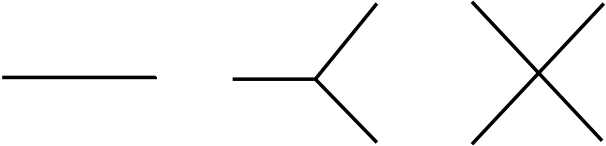
\includegraphics[width=10cm]{Feynman}
\end{figure}
The form of the propagator as well as the vertices can be derived from knowing the equations of motion/Lagrangian of classical GR. Graviton scattering amplitude can be computed by putting together the vertices and propagators in the usual fashion. 
\begin{figure}[h]\centering
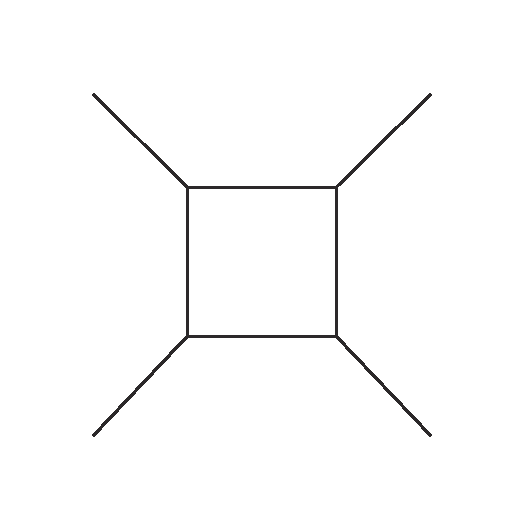
\includegraphics[width=4cm]{Divergence}
\end{figure}
Then, the loop diagrams has ultraviolet divergence, which cannot be removed by renormalization. Therefore, the renormalization procedure does not work for gravity. Naive quantization of GR does not give a consistent theory. String theory is an attempt to resolve this problem.

\subsection{Bosonic string theory}
The basic idea in string theory is different elementary particles are all vibrational modes of a single type of string. 
 If the typical size $\ell_s$  of a string is smaller than the resolution that an accelerator can provide, we cannot see this in the experiment involving elementary particles. To see the stringy nature of elementary particles, we need ``light'' of wavelength $\lambda<\ell_s$, i.e. energy $\frac{\hbar}{\lambda}c>\frac{\hbar}{\ell_s}c$. In the standard scenario, the string length is of order $\ell_s10^{-33}$ cm so that it requires $\frac{\hbar }{\ell_s}c \sim 10^{19}$ GeV, which is by far higher than $10^3$ GeV at LHC. At present day, experiments strings will appear to be point-like objects. Since, given  a string, there are infinitely many number of harmonic oscillators, there are infinitely many number of energy levels. Thus, it would appear that a string theory contains infinite numbers of elementary particles, which seems to contradict what we know about nature. However, most of these particles have mass of order $\frac{\hbar }{\ell_s}c \sim 10^{19}$ GeV so that they cannot be produced in the accelerator at present day. Only those states which have mass $<<\frac{\hbar }{\ell_s}c $ will be observable at current accelerators. One particular quantum state of the string presents a massless spin 2 particle. Recall that graviton is a massless spin 2 particle so that string theory automatically contains a graviton. However, before we can say that string theory contains gravity, we should see if this massless spin 2 particle interacts in the same way as a graviton. 



As interactions between point particles are determined by summing up Feynman diagrams, string interactions are described by summing over all surfaces between $A+B\to C+D$.
\begin{figure}[h]\centering
\includegraphics[width=5cm]{string-4}
\end{figure}
If we want scattering of strings in specific energy eigenstates (i.e. the graviton state) we need to take the convolution of the position space amplitude with the corresponding wave function. In this way, we can calculate the graviton scattering amplitude. When the energies of the external states are small compared to $\frac{\hbar }{\ell_s}c$, the 4-point scattering amplitude calculated from string theory agrees exactly with that calculated from tree level graphs in GR. This is also true for higher point amplitudes. Thus, the spin 2 particle in string theory has interaction exactly like that of the graviton. Note that in quantum general relativity,  the form of the vertex is fixed by the action giving the Einstein 's equation. In string theory, there is no vertex as the surface is smooth. We have no freedom in specifying how the strings should interact. Yet we get out an interaction that contains quantum GR. Thus in string theory quantum mechanics and principles of special relativity are inputs and GR is an output. 

What about the problem of ultraviolet divergences? The divergence comes when all four vertices come close to each other. What will be the corresponding diagram in string theory? This diagram has no vertices .Thus when we sum over all surfaces (we do not encounter configuration analogous to collapsed vertices. String theory amplitudes have no ultraviolet (shot distance) divergence.  As a result, string theory provides a finite quantum theory of gravity. Moreover, this is even better than renormalizable quantum field theories since here there is no divergence in the first place. 
\begin{figure}[h]\centering
\includegraphics[width=4cm]{string-loop}
\end{figure}

However, there are several caveats in bosonic string theory. (The string theory described here is called the bosonic string theory) First, this theory is consistent only when the number of spacetime dimensions is 26 (instead of 4).  Second, the graviton and other massless states, this theory contains a particle with negative mass${}^2$ called a \textbf{tachyon}. Third, this theory contains but not other known interactions  (string weak EM) in nature. Furthermore this does not have fermions. In conclusion, this does not look like the theory we observe in Nature.

The problem of not having gauge interaction can be resolved by including open strings in the theory. Just like the one of the states of a closed string represent a massless spin 2 particle and resembles a graviton, some of the modes of open string correspond to spin 1 particles and resembles non-Abelian gauge bosons in their interaction. But in order to resolve the other problems we need to turn to superstring theory.

\subsection{Superstring theory}





Strings besides vibrating in usual spacetime also has some internal degree of freedom. These internal degrees of freedom are fermionic. Thus a superstring could be regarded as a collection of infinite number of bosonic and fermionic harmonic oscillators. This can be quantized in a similar manner to that for bosonic strings. The good feature (e.g. emergence of gravity and UV finiteness) are preserved, but some (but not all) bad features disappear. 
\begin{enumerate}
\item the theory is consistent in 10 spacetime dimensions instead of 4. 
\item the tachyonic mode is absent
\item there are five fully consistent string theories in $d=10$. 

Type IIA, Type IIB, Type I (open+closed string), $E_8\times E_8$ heterotic, $SO(32)$ heterotic

\item the last 3 theories have non-Abelian gauge interaction besides gravity 
\item except for Type IIA, the other theories also contain Weyl (chiral) fermions. Recall that Nature contains chiral fermions like the neutrino. 
\item  all of these theories have a special kind of symmetry known as supersymmetry, which relates bosonic states to fermionic states and vice versa.
\item Furthermore all the five apparently different string theories have been found to be different limits of the same underlying theory called  M-theory
\end{enumerate}
Although this is closer to Nature compared to the bosonic string theory, we are still far from a realistic model. 

How do we reduce the number of dimensions from 10 to 4? The answer is Kaluza-Klein mechanism/compactification. As a toy example we shall start from a (1+1)-dimensional theory from there. Consider the two dimensional space to describe the surface of an infinite cylinder rather than an infinite plane.  If $R$ is much larger the range of the most powerful telescope, then the scientists living in the space will not know that they are living on a cylinder and not on a plane. If $R$ is not so large, then scientists with powerful telescopes will see it.  As $R$ becomes smaller and smaller more and more people can fell the effect. But now suppose $R$ is so small that it is smaller than the resolution of the most powerful microscope, then the space will look one-dimensional. Thus the same space in one limit may look 2-dimensional and in another limit may look one-dimensional. This is the same principle that can be used to make a (9+1) dimensional theory look (3+1)-dimensional. Take the 10-dimensional space of the form $\bR^{1,3}\times K$ where $K$ is a 6-dimensional compact space and its size is much smaller than resolution of most powerful microscopes (accelerator) $\sim 10^{-17}$cm. When $K$ is more than one-dimensional then there are many different possible choices for $K$. Not all of them are consistent (e.g. the metric does not satisfy Einstein equations). A certain subset of 6-dimensional manifolds satisfying all consistency requirements are known as Calabi-Yau manifolds. Taking $K$ to be a CY manifold gives four-dimensional theories with all the qualitative feature of the SM. For example, for a suitable choice of $K$ can get four-dimensional theories containing
\begin{enumerate}
\item Gravity
\item $SU(3)\times SU(2)\times U(1)$ gauge interaction
\item 3 generation of quarks and leptons including neutrinos which are Weyl fermions
\end{enumerate}
However so far nobody has found suitable manifold $K$ which gives exactly the SM with all the masses and coupling correctly. More importantly, there is as yet no theoretical principle for deciding which $K$ is chosen by Nature.




\subsection*{Convention}
$$\hbar=c=1~, \qquad \eta_{\mu\nu}=\textrm{diag}(-1,1,\cdots,1)~.$$

\section{Quantization of relativistic particles}
\subsection{Classical action}
Our aim will be to quantize a string consistent with the principles of quantum mechanics and special relativity. We shall do this in analogy with the quantization of relativistic point particle. To begin with, let us consider classical dynamics of relativistic point particle. The action of relativistic point particle is 
\be\label{action-particle}
S=c\int^b_ad\tau=c\int^b_a \Big( -\eta_{\mu\nu}\frac{dx^\mu}{d\tau}\frac{dx^\nu}{d\tau}\Big)^{\frac12}ds
\ee
whose the equation of motion is
$$
\frac{d}{ds}\left[\Big( -\eta_{\mu\nu}\frac{dx^\mu}{ds}\frac{dx^\nu}{ds}\Big)^{-\frac12}\frac{dx^{\nu}}{ds}\right]=0~.
$$
Using the change of variable
$$
\frac{d}{ds}=\Big( -\eta_{\mu\nu}\frac{dx^\mu}{ds}\frac{dx^\nu}{ds}\Big)^{\frac12}\frac{d}{d\tau}~,
$$
the equation motion can be written as
$$
\Big( -\eta_{\mu\nu}\frac{dx^\mu}{ds}\frac{dx^\nu}{ds}\Big)^{\frac12} \frac{d^2x^\mu}{d\tau^2}=0~.
$$
Therefore, the solution is 
\begin{align}
\textrm{massless particles}&:  ~\eta_{\mu\nu}\frac{dx^\mu}{ds}\frac{dx^\nu}{ds}=0\cr
\textrm{massive particles}&:  ~\frac{d^2x^\mu}{d\tau^2}=0\nonumber
\end{align}
Thus the action reproduces the right equation of motion. Our next task is to quantize it. This is made difficult by the square root in the action so that we first need to simplify it. To this end we replace the action \eqref{action-particle} by another action which is classically equivalent to the action \eqref{action-particle}, which gives the same equations of motion. Consider the following action
$$
S=\frac{c}2 \int ds \left[\Big( -\eta_{\mu\nu}\frac{dx^\mu}{ds}\frac{dx^\nu}{ds}\Big)^{\frac12}\lambda(s)+\lambda(s)^{-1}\right]
$$
Then,  $\lambda(s)$ plays a role of a Lagrangian multiplier
$$
\frac{\delta S}{\delta \lambda(s)}=0 ~\longrightarrow~ \lambda(s)^{-2}= -\eta_{\mu\nu}\frac{dx^\mu}{ds}\frac{dx^\nu}{ds}
$$
so that the substitution provides the action \eqref{action-particle}. Alternatively,  the derivative with respect to $x^\mu$ leads to the same equation of motion
$$
\frac{\delta S}{\delta x^\mu}=0 ~\longrightarrow~ \frac{d}{ds}\Big(\lambda(s)\eta_{\mu\nu}\frac{dx^\nu}{ds}\Big)=\frac{d}{ds}\left[\Big( -\eta_{\mu\nu}\frac{dx^\mu}{ds}\frac{dx^\nu}{ds}\Big)^{-\frac12}\eta_{\mu\nu}\frac{dx^{\nu}}{ds}\right]=0~.
$$
As a reinterpretation of the action, let us define $g_{ss}=\lambda(s)^{-2}$, which can be regarded as a $1\times 1$-matrix. Then, the action can be expressed as
$$
S=\frac{c}{2}\int ds \sqrt{\det{g_{ss}}} \left[ -g^{ss} \eta_{\mu\nu}\frac{dx^\mu}{ds}\frac{dx^\nu}{ds}+1\right]
$$
which is a one-dimensional general covariant action. Therefore, $g_{ss}$ is a metric in the space labelled by $s$, which is transformed as
$$
g_{ss} \to (f'(s))^{-2}g_{ss} \qquad \textrm{as} \  s\to f(s)~.
$$
Then, the transformation with $f'(s)=(g_{ss})^{-1/2}$ leads to the proper time $\tau$.

\subsection{Quantization of relativistic particle}
Since $S$ is a free field action, it is straightforward to quantize it. 
\begin{align}
p_\mu&=\frac{\partial S}{\partial(\partial_s x^\mu)}=-c~\eta_{\mu\nu}\frac{dx^\mu}{ds}\cr
H&=p_\mu\frac{dx^\mu}{ds}-L=-\frac{1}{2c}\eta^{\mu\nu}p_\mu p_\nu-\frac{c}{2}
\end{align}
Let us write a basis of momentum eigenstates by $|k\rangle$ so that $p_\mu|k\rangle=k_\mu|k\rangle$. The constraint is $\eta^{\mu\nu}p_\mu p_\nu=-c^2$. If $c=m$, this agrees with the expected property $\eta^{\mu\nu}p_\mu p_\nu=-m^2$ of a relativistic point particle. 


Light cone gauge is a different gauge fixing which destroys manifest covariance, but the constraints are easier to solve at the operator level. Because of
$$
 \eta_{\mu\nu}\frac{dx^\mu}{ds}\frac{dx^\nu}{ds}=\frac{dx^+}{ds}\frac{dx^-}{ds}-\sum_{i=2}^{d-2}\frac{dx^i}{ds}\frac{dx^i}{ds}~,
$$
the variation with respect to $x^+$ provides the equation of motion
$$
\frac{d}{ds}\Big(\lambda(s)\frac{dx^-}{ds}\Big)=0~.
$$
If we choose $s$ in such a way that $s=x^+=x^0+x^{d-1}$, the action can be written as 
$$
S=\frac{m}{2}\int ds\left[-\Big( \frac{dx^-}{ds}-\frac{dx^i}{ds}\frac{dx^i}{ds}\Big) \lambda(s)+\lambda(s)^{-1}\right]~.
$$ 
Since we have
$$
p_-=\frac{\delta S}{\delta (\partial_s x^-)}=\frac{m\lambda}{2}~, \quad p_\lambda=\frac{\delta S}{\delta (\partial_s \lambda)}=0~, \quad p_i=\frac{\delta S}{\delta (\partial_s x^i)}=-\lambda m \frac{dx^i}{ds}~,
$$
the hamiltonian can be expressed as
$$
H=p_-\partial_s x^-+p_\lambda \partial_s \lambda+p_i\partial_s x^i-S=-\frac{p_ip_i}{2m\lambda}-\frac{m}{2\lambda}=-\frac{p_ip_i}{4p_-}-\frac{m^2}{4p_-}~.
$$
The commutation relation can be worked out using the constrained Hamiltonian formalism.
$$
[x^-,p_-]=i~,\quad [x^i,p^j]=i\delta^{ij}~.
$$
The Hilbert space is spanned by
$$
e^{i(k_-x^-+k^ix^i)}:=|k_-,\vec k\rangle~,
$$
which are the eigenstates of momentum operators
$$
p_-|k_-,\vec k\rangle=k_-|k_-,\vec k\rangle`, \quad p^i|k_-,\vec k\rangle=k^i|k_-,\vec k\rangle~,
$$
where $k_-$ and $k^i$ are unconstrained variables. The Hamiltonian is
$$
H|k_-,\vec k\rangle=\Big(-\frac{k^ik^i}{4k_-}-\frac{m^2}{4k_-}\Big)|k_-,\vec k\rangle~.
$$
Thus, it admits a natural interpretation $H=-p_+$ which provides the usual relation
$$
k_+=\frac{k^ik^i}{4k_-}+\frac{m^2}{4k_-}~ 
$$

\subsection{Quantization of relativistic string}

The action is given by the area of a surface $\Sigma$ swept by a string
$$
S=-T\int_\Sigma \textrm{Area}~.
$$
where $T$ is the string tension. If we parametrize the surface by $(\xi^0,\xi^1)=(\sigma, \tau)$, then the action can be expressed as
$$
S=-T\int_\Sigma d^2\xi\sqrt{-\det (h_{\alpha\beta})}~,\qquad h_{\alpha\beta}=\eta_{\mu\nu}\partial_\alpha X^\mu\partial_\beta X^\nu.
$$
First we need to remove square root. An alternative action is 
$$
\wt S=-\frac T2\int d^2\xi \sqrt{-\det \gamma}~ \gamma^{\alpha\beta}\partial_\a X^\mu \partial_\b X^\nu \eta_{\m\n}
$$
where $\gamma_{\a\b}$ is 2 by 2 symmetric invertible matrix valued field. The equation of motion for $\gamma$ can be read off
$$
\delta \wt S=-\frac T2 \int d^2\xi\sqrt{-\det \gamma}~ \g^{\a\a'}\g^{\b\b'} \delta\gamma_{\alpha\beta}\Big[  \eta_{\m\n}\partial_{\a'} X^\mu \partial_{\b'} X^\nu -\frac12 \g_{\a'\b'}    \eta_{\m\n}\partial_{\s} X^\mu \partial^{\s} X^\nu \Big]
$$
where we use
\begin{align}
\delta(\sqrt{-\det \gamma})&=\frac12 (-\det \gamma)^\frac12 \gamma^{\a\b} \delta\gamma_{\a\b}\cr
\delta\gamma^{\a\b} &=-\g^{\a\a'}\delta \g_{\a'\b'}\g^{\b\b'}~
\end{align}
Therefore, the stress-energy tensor can be written as 
$$T_{\a\b} = \eta_{\m\n}\partial_{\a} X^\mu \partial_{\b} X^\nu -\frac12 \g_{\a\b} \;   \eta_{\m\n}\partial_{\s} X^\mu \partial^{\s} X^\nu~.$$
Then, 
$$\gamma_{\a\b}=F(\xi) ~ \eta_{\m\n}\partial_{\a} X^\mu \partial_{\b} X^\nu=F(\xi) ~h_{\a\b}$$
solves $T_{\a\b}=0$ for any function $F(\xi)$. Substituting $-\det \g=-F^2(\xi) \det h$ for the expression of $\wt S$,  we have
$$
\wt S=-T\int d^2\xi \sqrt{-\det \xi}
$$
so that $\wt S$ and $S$ describes the same action after we eliminate $\g_{\a\b}$ in $\wt S$ by its equation of motion. 


\subsubsection*{Symmetry of $\wt S$}
\begin{enumerate}
\item\textbf{Re-parametrization invariance}

Under the re-parametrization
\begin{align}
\wt X^{\mu}(\vec\xi')&=X^{\mu}(\vec\xi)\quad \textrm{with}\quad  \vec{\xi'}=\vec{f}(\xi)~,\cr
\wt \g_{\a\b}&=\g_{\d\g}\frac{\partial\xi'^\a}{\partial\xi^\d}\frac{\partial\xi'^\b}{\partial \xi^\g}~,\nonumber
\end{align}
the action is invariant $\wt S(X^\m,\g_{\a\b})=\wt S(\wt X^\m,\wt\g_{\a\b})$. We have two parameter family of gauge symmetry.
\item\textbf{Weyl invariance}

The action is also  invariant under the metric $\wt \g_{\a\b}=e^{\phi(\xi)}\g_{\a\b}$ by an arbitrary function $\phi(\xi)$. This symmetry is called the \emph{Weyl symmetry}.
\item\textbf{Lorentz transformation}

The action is certainly invariant under the Lorentz transformation
$\wt X^\mu(\xi)=\L^\mu{}_\nu X^\nu(\xi)$ where $\L\eta\L^T=\eta$.
\end{enumerate}


We can fix these of the $d+3$ fields $X^\mu$ and $\g_{\a\b}$. We have different possible choices, but we choose covariant gauge fixing $\gamma_{\a\b}=\eta_{\a\b}=\textrm{diag}(-1,1)$. In the covariant gauge, the action can be written as a free field 
$$
\wt S=-\frac T2 \int d^2\xi ~\eta^{\a\b} \eta_{\m\n}\partial_{\a} X^\mu \partial_{\b} X^\nu~.
$$
The equation of motion constraints 
$$
0=T_{\a\b} = \eta_{\m\n}\partial_{\a} X^\mu \partial_{\b} X^\nu -\frac12 \eta_{\a\b} \;   \eta_{\m\n}\partial_{\s} X^\mu \partial^{\s} X^\nu~.
$$
One of the three constraints is redundant and the independent constraints are
\begin{align}
T_{uu}= \frac1{\a'}  \eta_{\m\n}\partial_{u} X^\mu \partial_{u} X^\nu=0~, \qquad
T_{vv}= \frac1{\a'} \eta_{\m\n}\partial_{v} X^\mu \partial_{v} X^\nu=0~.
\end{align}
where $u=\tau+\sigma$

For the quantization of relativistic string, we first quantize the free scaler field theory of the $X^\mu$ and next impose the physical state condition 
\be\label{constraint}
\langle \textrm{phys}'| T_{uu}| \textrm{phys} \rangle =0 \qquad  \langle \textrm{phys}'| T_{vv}| \textrm{phys} \rangle =0 ~.
\ee

For closed string theory, we impose the periodic boundary condition $X^\mu(\s+2\pi ,\tau)=X^\mu(\s,\t)$ so that we expand
$$
X^\mu(\s,\t)=x^\mu+\sum_{n\neq 0} \phi_n^\mu(\t)e^{in\s}~.
$$
Substituting this into the action, we have a collection of harmonic oscillators
$$
\wt S=T\pi \Big[\eta_{\mu\nu} \partial_{\t} x^\mu \partial_{\t} x^\nu+ \sum_{n? 0}\eta_{\mu\nu}( \partial_{\t} \phi_{-n}^\mu \partial_{\t} \phi_{n}^\nu-n^2  \phi_{-n}^\mu \phi_{n}^\nu )\Big] ~.
$$
We can define the conjugate variable to $x^\nu$ and $\phi_n^\nu$
$$
\Pi_{\nu n}=\frac{\delta \wt S}{\delta (\partial_\t \phi^\nu_n)} =\frac{1}{\a'}\eta_{\mu\nu}\partial_\t \phi^\mu_{-n}~, \qquad p_\n=\frac{\delta \wt S}{\delta (\partial_\t x^\nu)} =\frac{1}{\a'}\eta_{\mu\nu}\partial_\t x^\mu~,
$$
which satisfy the following commutation relation
$$
[x^\m,p_\n]=i\delta^\m_\n\qquad [\phi_n^\nu,\Pi_{\nu m}]=i\delta^\n_\m\delta_{m,n}~.
$$
The Legendre transformation defines the Hamiltonian
\begin{align}
H&=p_\n\partial_\t x^\nu +\sum_{n\neq 0} \Pi_{\n,n} \partial_\t \phi^\nu_n- \wt S\cr
&=\frac{\a'}{2}\eta^{\m\n}p_\m p_\n +\a'\sum_{n\neq 0} \eta^{\m\n}\Pi_{\m,-n}\Pi_{\n,n} +\frac1{\a'}\sum_{n\neq 0}n^2   \eta_{\m\n}\phi_{-n}^\mu \phi_{n}^\nu
\end{align}
where $T=1/(2\pi \a')$.

We define
\begin{align}
&\a_{-n}^\m:=\frac1{\sqrt{2}}\Big[\sqrt{\a'}\eta^{\m\n}\Pi_{\n n}+\frac{i n}{\sqrt{\a'}} \phi_{-n}^\m\Big]\qquad (\a_{-n}^\m)^\dagger =\a_{n}^\m\cr
&\wt\a_{n}^\m:=\frac1{\sqrt{2}}\Big[\sqrt{\a'}\eta^{\m\n}\Pi_{\n n}-\frac{i n}{\sqrt{\a'}} \phi_{-n}^\m\Big]\qquad (\wt\a_{n}^\m)^\dagger =\wt\a_{-n}^\m
\end{align}
and then they satisfy the commutation relation
$$
[\a_{-m}^\m,\a_{-n}^\m]=m\delta_{m+n,0}\eta^{\m\n}\qquad  [\wt\a_{m}^\m,\wt\a_{n}^\m]=m\delta_{m+n,0}\eta^{\m\n} \qquad  [\a_{m}^\m,\wt\a_{n}^\m]=0~.
$$
Then, the Hamiltonian can be written as
$$
H= \textrm{const}+\frac{\a'}{2}\eta^{\m\n}p_\m p_\n +\sum_{n>0} \eta_{\m\n} (\a_{-n}^\m\a_{n}^\n+\wt \a_{-n}^\m\wt \a_{n}^\n)
$$
where the constant part comes form the normal ordering. The creation operators are $\a_{-n}^{\m},\wt \a_{-n}^{\m}$ and the annihilation operators are $\a_{n}^{\m},\wt \a_{n}^{\m}$ for $n\in\bN$ so that the Hilbert space is spanned by
$$
\a_{-n_1}^{\m_1}\cdots \a_{-n_k}^{\m_k} \wt\a_{-n_1}^{\m_1}\cdots \wt\a_{-n_k}^{\m_k}|k\rangle   \qquad \textrm{where} \qquad p^\m|k\rangle=k^\m|k\rangle~.
$$


The stress-energy tensor admits the decomposition
$$
T_{uu}=\a'\sum_n L_ne^{in\sigma} \qquad T_{vv}=\a'\sum_n \wt L_ne^{-in\sigma}
$$
where 
\begin{align}
L_m&=\sqrt{\frac{\a'}{2}}\a^\m_m p_\m+\frac12 \sum_{n\neq0} \eta_{\m\n} \a^\m_{m-n}\a^\n_n \qquad L_0=\textrm{const}+\frac{\a'}{4}p^\m p_\m+\frac12 \sum_{n>0} \eta_{\m\n} \a^\m_{-n}\a^\n_n\cr
\wt L_m&=\sqrt{\frac{\a'}{2}}\wt \a^\m_m p_\m+\frac12 \sum_{n\neq0} \eta_{\m\n} \wt \a^\m_{m-n}\wt \a^\n_n \qquad L_0=\textrm{const}+\frac{\a'}{4}p^\m p_\m+\frac12 \sum_{n>0} \eta_{\m\n} \wt \a^\m_{-n}\wt \a^\n_n\
\end{align}
The constraint \eqref{constraint} on the stress-energy tensor can be defined by
\begin{align}
L_n| \textrm{phys} \rangle =0 \qquad \wt L_n| \textrm{phys} \rangle =0 \qquad \textrm{for} \quad n\ge0\cr
\langle \textrm{phys}'|L_{-n}  =0 \qquad \langle \textrm{phys}'|\wt L_{-n}=0 \qquad \textrm{for} \quad n\ge0
\end{align}
so that
$$
\langle \textrm{phys}'| L_n | \textrm{phys} \rangle =0 \qquad  \langle \textrm{phys}'| \wt L_n | \textrm{phys} \rangle =0 ~.
$$







































\end{document}




